\section{Aufbau des Plugins}\label{AUFBAUPLUGIN}
In diesem Kapitel wird der grundsätzliche Aufbau eines Plugins besprochen. Dabei werden neben allgemeinen Details, wie die Aktivierung eines Plugins, auch einzelne Programmierdetails angesprochen. Inbegriffen sind hierbei der erste Abschnitt eines jeden Plugins: der \nameref{ACHE}, sowie die einzelne Funktionen und wie diese referenziert werden.
\subsection{Allgemeines}
Ein paar Details zur Programmierung von Plugins wurden bereits im Unterkapitel \ref{WIEP} angesprochen - beispielsweise eine Einleitung zu hooks.\newline
Nach Hetzel\footcitetgedr[Vgl.][Seite 274]{AH12} gibt es jedoch einige technische Details, mit welchen sich der Programmierer beschäftigen muss, bevor die eigentliche Programmierung beginnen kann. Zunächst ein Detail, welches auch in \nameref{WIEP} angesprochen wurde, jedoch von außerordentlicher Wichtigkeit ist: Plugins werden generell unter Wordpress in dem Plugin-Ordner {\emph{/wp-content/plugins/}}. Dies hat den wichtigen Grund, dass Wordpress nur Plugins erkennt, welche auch in diesem Ordner kopiert worden sind. Weiterhin bietet es sich an, für jedes Plugin einen eigenen Unterordner zu erstellen, um so die Übersichtlichkeit bei dem Einsatz mehrerer Plugins zu gewährleisten. Auch sollte die Hauptdatei des Plugins immer den Namen des Plugins haben und eine Namenskonvention, welche nicht mit anderen Plugins in Konflikt kommt, eingehalten werden.\newline
An dieser Stelle möchten wir vorstellen, wie die Details für das Plugin Mentoren-Suche aussehen:
\begin{enumerate}
	\item Als Hauptordner unter dem Pluginverzeichnis {\emph{/wp-content/plugins}} haben wir {\emph{mentoren-suche}} gewählt 
	\item Die Hauptdatei unseres Plugins lautet {\emph{mentoren-suche.php}}
\end{enumerate}
Soviel zu den Details für die Vorbereitung der Programmierung. Im nächsten Abschnitt wird erläutert, wie das Plugin aktiviert wird.
\subsection{Aktivierung des Plugins}\label{aktivierungplugin}
Insgesamt gibt es aus Anwendersicht drei Schritte\footcitetgedr[Vgl.][Seite 29]{BB11}, um ein Plugin zu aktivieren:
\begin{enumerate}
	\item Als erster Schritt wird zum Wordpress Dashboard navigiert ({\emph{http://localhost/wp-admin/} oder \emph{http://deine-domain/wp-admin/}})
	\item Anschließend wird die Option {\emph{Plugins}} ausgewählt
	\item Als letzter Schritt wird auf {\emph{Aktivieren}}	des entsprechenden Plugins ({\emph{mentoren-suche}}) geklickt
\end{enumerate}
Soviel einmal zur Theorie. Der nächste Abschnitt leitet in die Praxis der Aktivierung.
   \begin{figure}[htbp]
	\begin{center}
		
\includegraphics[angle={360}, scale=0.61]{pictures/plugin_deak.jpg}
	    \caption{Pluginübersicht im Pluginmenü}
	    \label{img:ERFMELDPM}
	    	\end{center}
   \end{figure} 
Zur besseren Übersichtlichkeit und für eine ersten Eindruck des fertigen Plugins, ist in Abbildung 
\ref{img:ERFMELDPM} das Pluginmenü mit den entsprechenden Informationen aus dem im nächsten Unterkapitel \nameref{ACHE} abgebildet.
   \begin{figure}[htbp]
	\begin{center}
	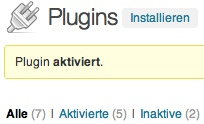
\includegraphics[angle={360}, scale=0.61]{pictures/plugin_akt.jpg}
	    \caption{Erfolgreiche Meldung der Aktivierung}
	    \label{img:ERFMELDAK}
	\end{center}
   \end{figure}\newline
Nach einem Klick auf \emph{Aktivieren} ist das Plugin aktiviert und es erscheint die in Abbilung \ref{img:ERFMELDAK} abgebildete Meldung.
Während der Aktivierung werden verschiedene Funktionen ausgeführt. Beispielsweise wird im Backend-Menü in der Menüstruktur angelegt oder es wird geprüft, ob die benutzte Wordpressversion mit dem Plugin kompatibel ist. Weiterhin steht auch nun der Shortcode für das Plugin bereit und die Übersetzungen der einzelnen Textelemente werden angezeigt. \newline
Wie dies alles zu programmieren ist, wird in dem nächsten Kapiteln besprochen. Dabei wird als erstes auf den Informationen Header, anschließend auf einzelne Funktionen und abschließend die Hooks besprochen. Soviel erst einmal zur Aktivierung und kleinen technischen Hintergrundabläufen. 
\subsection{Information Header}\label{ACHE}
In Wordpress ist der {\emph{Information Header}} in der Pluginentwicklung immer der erste Teil des Programmes. Er wird dafür benötigt, um im Pluginmenü erforderliche Informationen über den Autoren oder eine Beschreibung des Plugins darzustellen - wie bereits im Unterkapitel \nameref{aktivierungplugin} dargestellt ist. Ohne diesen Header wird kein Plugin funktionieren, auch wenn die Programmierung bis in kleinste Detail abgeschlossen ist.\footcitetgedr[Vgl.][Seite 30]{BB11} \newline
Wie ein solcher aussehen könnte, ist beispielhaft in Listing \ref{CINHEA} dargestellt. Dabei handelt es sich immer um eine Angabe, welche in Kommentaren geschrieben wird (\emph{/*}).
\lstset{language={PHP},caption={Information Header},label=CINHEA}
\begin{lstlisting}
<?php
/*
Plugin Name: Mentoren-Suche
Description: Suchfunktion der Mentoringgruppe f&uuml;r Mentees
Version: 1.0
Author: Timo Amling, Ludger Sch&ouml;nfeld, Anatol Tissen im Auftrag von Mentoring4Excellence (FH K&ouml;ln, Campus Gummersbach - Programmleitung: Frau Prof. Dr. Gabriele Koeppe)
- im August 2012
License: GPL 3
*/
...
?>
\end{lstlisting}
Wie sich erkennen lässt, umfasst der Header insgesamt fünf Informationsobjekte. Zu den hier vorgestellten kann optional auch noch die Plugin-URL\gls{URL} - also falls das Plugin auf einer Website im Internet angeboten wird - angegeben werden.\footcitetgedr[Vgl.][Seite 31]{BB11}
Da es sich bei den Lesern dieses Tutorials größtenteils um Personen handelt, welche mit Informatik beruflich oder privat zu tun haben, wird hier nicht näher auf die einzelnen Objekte eingegangen.\newline
Im nächsten Kapitel werden erste Funktionen erzeugt, diese eingebunden und auf Fehler aufmerksam gemacht. 
\subsection{Benutzerdefinierte Funktionen}\label{benutzerdeffunkt}
In diesem Kapitel geht es darum, die ersten benutzerdefinierten Funktionen zu schreiben und auf mögliche Fehlerursachen aufmerksam zu machen. Dabei wird davon ausgegangen, dass eine korrekte php-Konfiguration vorhanden und der entsprechende Debug-Modus aktiviert ist. Wir möchten an dieser Stelle nur auf das Wordpress-System eingehen und  nicht auf externe Konfigurationsmöglichkeiten, da dies den Umfang dieses Tutorials sprengen würde. Weitere Informationen sind jedoch unter \url{http://php.net/manual/en/debugger.php} zu finden.
\subsubsection{Das erste eigene Plugin}
Als unsere erste Funktion soll eine normale Textausgabe mit folgendem Inhalt geschrieben werden \emph{Ich bin eine Textausgabe}. Dafür eignet sich der Befehl \emph{print}. Dieser ist bereits in Listing \ref{CERPRAU} eingefügt worden und kann anschließend im Pluginmenü von Wordpress aktiviert werden. Benutzerdefinierte Funktionen werden in Wordpress dafür benötigt, um Logik des Plugins zu programmieren (näheres dazu findet sich im Kapitel \ref{aktivierungplugin}).\footcitetgedr[Vgl.][Seite 35-36]{BB11}
\lstset{language={PHP},caption={Erste Printausgabe},label=CERPRAU}
\begin{lstlisting}
<?php
/*
Plugin Name: Mentoren-Suche - Printausgabe
Description: Ein erster Versuch
Version: 0.1
//...WEITERE ANGABEN VON INFORMATION-HEADER...
*/
print "Ich bin eine Textausgabe";
?>
\end{lstlisting} 
Nach der Aktivierung dieses Plugins erscheint im oberen Bereich der Plugin- und jeder anderen Seite der Back- und Frontendseite der entsprechender Text (vgl. Abbildung \ref{img:PRBEAUS}). 
\newpage
 \begin{figure}[!htbp]
	\begin{center}
		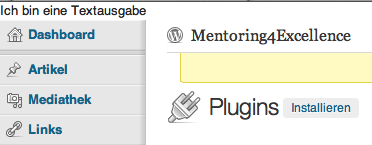
\includegraphics[angle={360}, scale=0.61]{pictures/printheader.png}
	    \caption{Printbefehl-Ausgabe}
	    \label{img:PRBEAUS}
	    	\end{center}
   \end{figure}
Dieses Verhalten ist darauf zurückzuführen, dass das Plugin nach dem aktivieren direkt geladen wird und so auf jede Seite vorhanden ist.\newline
Dies lässt sich durch das Hinzufügen von Funktionen unterbinden, welches in Listing \ref{VEBEBEI}, Zeile 8 - 10 dargestellt ist. 
\lstset{language={PHP},caption={Verbesserte Printausgabe},label=VEBEBEI}
\begin{lstlisting}
<?php
/*
Plugin Name: Mentoren-Suche - Printausgabe 2
Description: Ein zweiter Versuch
Version: 0.2
//...WEITERE ANGABEN VON INFORMATION-HEADER...
*/
function printausgabe(){
	print "Ich bin eine Textausgabe";
}
?>
\end{lstlisting} 
Das nun verwendete Plugin bewirkt, dass das Printstatement so isoliert wird, dass es erst bei unmittelbaren Aufruf verwendet wird. \newline
Zwar ist nach dem Aktivieren des Plugins das Textfeld verschwunden, allerdings taucht es dieses auch nicht an anderer Stekke auf. Dafür werden sogenannte Hooks (siehe Abschnitt \ref{sub_acvsfs}) verwendet.\footcitetgedr[Vgl.][Seite 38-39]{BB11} \newline
Bevor diese allerdings angesprochen werden und nach diesem kleinen Exkurs auch mit dem Mentoring-Plugin weitergearbeitet wird, wird im nächsten Kapitel \ref{subsub_debmod} noch die Aktivierung des Debug-Modus kurz erläutert.
\subsubsection{Debug-Modus}\label{subsub_debmod}
Es ist ratsam bei der Pluginentwicklung
 im sogenannten-Debug-Modus von Wordpress zu arbeiten, um so  Fehlermeldungen zu sehen und diese zu beheben.
Dieser Modus lässt sich in der Hauptkonfigurationsdatei \emph{wp-config.php} einstellen. Dafür muss im folgenden Listing der Wert in Zeile 9 von \emph{false} (ausgeschaltet) auf \emph{true} (eingeschaltet) geändert werden.\footcitetgedr[Vgl.][Seite 23]{BB11}
\lstset{language={PHP},caption={Debug-Modus aktivieren},label=CERPRAU}
\begin{lstlisting}
...
/**
 * For developers: WordPress debugging mode.
 *
 * Change this to true to enable the display of notices during development.
 * It is strongly recommended that plugin and theme developers use WP_DEBUG
 * in their development environments.
 */
define('WP_DEBUG', true);
...
\end{lstlisting} 
Nachdem der Debug-Modus aktiviert wurde, kann als Kontrolle nochmal die Funktion aus Listing \ref{CERPRAU} aktiviert werden. Anschließend wird zwar wieder im oberen Bereich die entsprechende Textausgabe ausgegeben, allerdings werden darunter einige Fehlermeldungen und Warnungen angezeigt: Der Debugger ist also aktiviert (siehe Abbildung \ref{img:PRMAKDE}). \newline
Wie dieser Fehler behoben wird ist an dieser Stelle schon aus Listing \ref{VEBEBEI} bekannt: Nämlich die Printausgabe als Funktion schreiben.\newline
 \begin{figure}[htbp]
	\begin{center}
		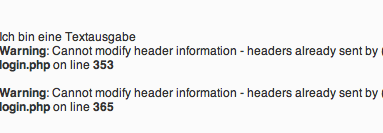
\includegraphics[angle={360}, scale=0.61]{pictures/printheadermeldung.png}
	    \caption{Printbefehl mit aktivierten Debugger}
	    \label{img:PRMAKDE}
	    	\end{center}
   \end{figure}\newline
Nachdem die Vorbereitungen abgeschlossen und die ersten Funktionen geschrieben wurde, wird nun das Referenzieren von Hooks über Filter und Actions angesprochen. 
\subsection{Hooks}\label{sub_acvsfs}
In diesem Kapitel wird sich mit sogenannten \emph{Hooks} beschäftigt. Diese sind dafür verantwortlich, wann ein Plugin ausgeführt ist. 
Genauer gesagt handelt es sich bei einem Hook um eine Art Eventhandler: Wenn ein bestimmtes Ereignis auftritt, wird eine gewisse Funktion ausgeführt. Ein solches Ereignis könnte beispielsweise vorliegen, wenn ein bestimmtes Menü angeklickt wird oder ein Suchfeld aktiviert wird.\newline
Dabei sollte noch erwähnt werden, dass sich diese Eventhandler in zwei Komponenten unterteilen lässt:Action- und Filter-Hooks.\footcitetgedr[Vgl.][Seite 39]{BB11}\newline
Wie diese genau funktionieren und allgemein aufgebaut sind, wird in den nächsten Abschnitten erläutert.

\subsubsection{Referenzieren mittels add\_action() und add\_filter()}\label{refmitaddacunaddfilt}
Bevor die eigentlichen Anwendungsbeispiele kommen, soll an dieser Stelle zuvor die allgemeine Syntax von \emph{action-} und \emph{filter}-Hooks erläutert werden:
\begin{table}[ht]
\centering
\begin{tabular}[h]{|l|c|c|c|c|c|}
\hline
\textbf{Hook-Art} & \textbf{Syntax} \\
\hline
Action & add\_action('Event','Funktion') \\
Filter & add\_filter('Event','Funktion') \\
\hline
\end{tabular}
\caption{Vergleich Action- und Filter-Hooks}
\label{tab:vglactufilhooks}
\end{table}
Anhand von Tabelle \ref{tab:vglactufilhooks} lässt sich erkennen, dass die beiden Hook-Arten genau gleich aufgebaut sind. Wie immer steckt hier der Teufel im Detail - genauer gesagt: Wie Wordpress mit diese beide Arten umgeht.\newline
Wenn eine Funktion zu einem Action-Hook verbunden wird, ignoriert die Funktion Eingabeparameter wie beispielsweise übergebene Variablen. Auch wenn die Funktion einen Rückgabewert besitzt, wird auch dieser Wert ignoriert.\footcitetgedr[Vgl.][Seite 40]{BB11} \newline
Dies ist der Punkt, an dem der Unterschied zum Filter-Hook klar wird: Dieser akzeptiert Eingabeparameter und Werte und kann diese verändert - oder eben gefiltert - zurückgeben.\newline
 Dies geschieht noch bevor dieser Parameter dem Benutzer auf dem Bildschirm angezeigt oder in die Wordpress-Datenbank geschrieben wird\footcitetint[Vgl.][]{MMTPA12}.\newline
 Im Grunde genommen haben die beiden Funktionen eines gemeinsam: Beide binden eine Event an eine Funktion, gehen nur jeweils anders damit um.\footcitetgedr[Vgl.][Seite 40]{BB11}\newline
  Eine überschaubare Funktionsreferenz von Action und Filter-Hooks lässt sich unter \url{http://codex.wordpress.org/Plugin_API} finden.
  
 \subsubsection{Hook-Anwendungsbeispiele}
 An dieser Stelle werden nun ein paar Beispiele aus dem Mentoren-Plugin genommen und weitestgehend erläutert. Anschließend wird noch eine weitere Funktion vorgestellt: Der add\_option-Hook.
\paragraph{Vordefinierte Actions}\ \newline
Wordpress bietet von Hause aus schon vordefinierte Actions, welche ab Wordpressversion 2.1 vorhanden und verwendbar sind. Da die Anzahl dieser vordefinierten Actions ziemlich umfangreich ist, wird an dieser Stelle nur auf ein Action verwiesen, welches vergleichbar oft in dem Mentorenplugin vorkam: Die Action \emph{add\_action}.\footcitetint[Vgl.][]{MMTPA12}

\lstset{language={PHP},caption={Beispiele für add\_action()},label=CADAC}
\lstset{
 morekeywords={add_action}
}
\begin{lstlisting}
<?php
...
add_action('admin_menu', 'register_Mentees_menu');
...
<?
\end{lstlisting}
An dieser Stelle wird auf die in Listing \ref{CADAC} vorgestellten Funktionen genauer eingegangen. \newline
Allgemein lässt sich formulieren, dass die Action \emph{admin\_menu} dafür verwendet wird, um ein zusätzliches Untermenü und bestimmte Menü-Optionen im Administrator-Bereich anzulegen.\footcitetint[Vgl.][]{MMTAR12}
Dies bedeutet, dass beim Aktivieren des Plugins verschiedene Actions ausgeführt werden. Beispielsweise wird eine Funktion \emph{register\_Mentees\_menu} aufgerufen, welche für die Erstellung des Submenüs zur Verwaltung des Plugins geschrieben wurde. \newline
Weitere Informationen werden zu diesem Thema im Kapitel \ref{Formular} angesprochen.

\paragraph{Eigene Actions}\ \newline
Natürlich ist es auch möglich eigene Actions zu schreiben und diese einer Menüstruktur zuordnen. Im Listing \ref{CADAC} sind solche Beispiele aufgelistet.
\lstset{language={PHP},caption={Beispiele für eigene add\_action()},label=CADAC}
\lstset{
 morekeywords={add_action}
}
\begin{lstlisting}
<?php
...
//wenn check erfolgreich, werden DB-Tabellen angelegt
add_action('hk_mentees_db_create','mentees_db_create');
add_action('hk_mentor_db_create','mentor_db_create');
...
<?
\end{lstlisting}
Falls also ein Mentor oder Mentee angelegt werden soll, werden die entsprechenden Daten wie Vor- oder Nachname in ein Formular eingetragen. Anschließend wird mit einem Button die Eingabe bestätigt. Genau das ist der Zeitpunkt, an dem die Action eintritt: Es muss eine Datenbank angelegt werden. Dies geschieht über die beiden Funktionen \emph{mentor\_db\_create} und \emph{mentees\_db\_create}. \newline
Wie mit solchen Datenbankobjekten interagiert wird, wird genau in Kapitel \ref{DBzugriff} besprochen.
\paragraph{Vordefinierte Filter}\ \newline
Da in dem aktuellen Plugin der Mentoren-Suche keine Filter zum Einsatz kommen, aber trotzdem für ein solches Tutorial von Bedeutung sind, wird an dieser Stelle auf Fachliteratur zurückgegriffen und entsprechend erläutert. \newline
Wie schon erläutert, handelt es sich bei Filter-Hooks um Funktionen, damit Wordpress bestimmte Text oder weitere Typen modifizieren kann.\newline
Nach Bondari und Griffiths\footcitetgedr[Vgl.][Seite 42 - 43]{BB11} soll das Ziel dieses kleinen Beispiel-Plugins nur verdeutlichen, wie Actions im Zusammenhang mit Filtern funktionieren. Dafür wird eine Kopie des Standard-Plugins \emph{hello dolly von Wordpress} verwendet und verändert. \newline
Die dazugehörige Plugindatei liegt im Pluginverzeichnis von Wordpress und lautet \emph{hello.php}
\lstset{language={PHP},caption={Beispiele für add\_filter()},label=CADFI}
\lstset{
 morekeywords={add_filter}
}
\begin{lstlisting}
<?php
...
//VORHER
add_filter('admin_footer','hello_dolly');

//NACHER
add_filter('the_content','hello_dolly');
...
<?
\end{lstlisting}
Wie in Listing \ref{CADFI} dargestellt, wird als Vorbereitung das Event von \emph{admin\_footer} auf \emph{the\_content} geändert, da hier die bisherigen Posts verändert werden sollen.\newline
Dafür wird in der Datei \emph{hello.php} zusätzlich auch die Funktion \emph{hello\_dolly()} verändert. \newline
Dies ist in Listing \ref{CAHD} genauer dargestellt.
\lstset{language={PHP},caption={Funktion \emph{hello\_dolly} mit Input-Variable},label=CAHD}
\lstset{
 morekeywords={add_filter}
}
\begin{lstlisting}
<?php
...
//VORHER
function hello_dolly() {
	$chosen = hello_dolly_get_lyric();
	echo "<p id='dolly'>$chosen</p>";
}

//NACHER
function hello_dolly($input) {
	$chosen = hello_dolly_get_lyric();
	return $input . "<p id='dolly'>$chosen</p>";
}
...
<?
\end{lstlisting}
Was hier nun passiert, lässt sich wie folgt beschreiben: Die Variable \emph{\$input} beschreibt den Inhalt eines jeden Posts. Dieser wird anschließend in die Filter-Funktion übertragen, modifiziert und anschließend per \emph{return} zurückgegeben.\newline
Anstatt die kompletten Inhalt eines Posts zu überschreiben, wird stattdessen ein beliebiger Text unterhalb des Posts eingebunden. Damit wird also schlussendlich der Inhalt verändert und dargestellt - genau das, was eine Filter-Funktion machen sollte.\newline
Unterm Strich lässt sich formulieren, dass eine Funktion, die bei einer Action aktiviert wird, keine Eingabe- und Ausgabewerte akzeptiert. \newline
Eine Action, die über eine Filter-Funktion aufgerufen wird, erlaubt die oben genannten Einschränkungen. Dies ist zugleich der Unterschied zwischen diesen beiden Event-Typen.\footcitetgedr[Vgl.][Seite 43]{BB11}
Weitere Informationen finden sich unter den folgenden Internetseiten zu finden:
\begin{enumerate}
	\item \url{http://codex.wordpress.org/Function\_Reference}
	\item \url{http://codex.wordpress.org/Action\_Reference}
\end{enumerate}
\paragraph{Funktion add\_option}\ \newline
Zum Schluss dieses Kapitels wird sich noch mit dem \emph{add\_option}-Hook beschäftigt. Dieser ist mehrmals im Plugin zum Einsatz gekommen und ist syntaktisch auch anders aufgebaut als ein \emph{filter} oder \emph{action}-Hook.\newline
Laut Mullenweg\footcitetint[Vgl.][Artikel Function Reference/add option]{MMTFR12} wird eine add\_option-Funktion dafür verwendet, um Optionen in die Wordpress-Datenbank zu schreiben.
Als erstes wird dabei geprüft, ob eine Funktion mit demselben Namen schon vorhanden ist. In diesem Fall wird ein \emph{false}  zurückgegeben.\newline
Wenn anschließend der Name keiner der geschützten Optionen überschreiben soll, wird die Option erstellt. Dies ist der allgemeine Ablauf, der sich hinter \emph{add\_option} befindet. Die allgemeine Syntax sowie ein Anwendungsbeispiel lässt sich aus Listing \ref{CADOP} ablesen.\newline
\lstset{language={PHP},caption={Beispiele für add\_option()},label=CADOP}
\lstset{
 morekeywords={add_option}
}
\begin{lstlisting}
<?php
...
//Allgemeine Syntax 
add_option('Option','Value','Deprecated','autoload')
//Beispiel
add_option('ms_frontend_searchform_url','','',yes);

<?
\end{lstlisting}
In dem in Listing \ref{CADOP} dargestellten Beispielen muss ergänzt werden, dass die Werte \emph{Value} (für Option-Name reserviert), \emph{deprecated} (nur für Wordpressversion 2.3) und \emph{autoload} (ob die Funktion automatisch geladen werden soll mit Standardwert \emph{yes} für ja) optional sind.\newline
Im konkreten Anwendungsbeispiel wird also die Option \emph{ms\_frontend\_searchform\_url} aufgerufen und in die Datenbank eingetragen. Diese Option ist dafür verantwortlich, dass im Frontendbereich an der Stelle, an dem der Shortcode eingebunden wird (ausführlich im nächsten Kapitel), eine Suchmaske erscheint und ausgeführt werden kann.\newline
Wie diese aussieht, wird im nächsten Kapitel näher besprochen.\newline
Soviel zu den Hooks. Im nächsten Kapitel \ref{shortcodes} wird die Thematik \nameref{shortcodes} behandelt.